% Created 2024-03-07 Thu 18:23
% Intended LaTeX compiler: pdflatex
\documentclass[a4paper, 12pt]{article}
\usepackage[utf8]{inputenc}
\usepackage[T1]{fontenc}
\usepackage{graphicx}
\usepackage{longtable}
\usepackage{wrapfig}
\usepackage{rotating}
\usepackage[normalem]{ulem}
\usepackage{amsmath}
\usepackage{amssymb}
\usepackage{capt-of}
\usepackage{hyperref}
\usepackage[utf8]{inputenc}      % accents
\usepackage[T1]{fontenc}         % PS fonts
\usepackage{newtxtext,newtxmath} % do not use CM fonts
\usepackage{amsmath}             % multi-line and other mathematical statements
\usepackage{setspace}            % setting the spacing between lines
\usepackage{graphicx}            % go far beyond what the graphics package
\usepackage[normalem]{ulem}      % various types of underlining
\usepackage{caption}             % rotating captions, sideways captions, etc.
\usepackage{float}               % tables and figures in the multi-column environment
\usepackage{subcaption}          % for subfigures and the like
\usepackage{longtable}           % tables that continue to the next page
\usepackage{multirow}            % tabular cells spanning multiple rows
\usepackage[table]{xcolor}       % driver-independent color extensions
\usepackage{lipsum}              % loren dummy text
\setlength{\marginparwidth}{2cm} % todonotes' requirements
\usepackage{todonotes}           % todo's
\usepackage{chicago}             % a bibliography style
\usepackage{bookmark}            % Include the bookmark package
\usepackage[a4paper,left=25mm,right=25mm,top=25mm,bottom=25mm,headheight=6mm,footskip=12mm]{geometry}
\setlength{\parindent}{0em}
\setlength{\parskip}{4ex}
\AddToHook{cmd/section/before}{\clearpage}
\usepackage{fancyhdr}
\fancyhf{}                            % clear off all default fancyhdr headers and footers
\rhead{\small{\emph{\projtitle, \projauthor}}}
\rfoot{\small{ \thepage\ }}
\pagestyle{fancy}                     % apply the fancy header style
\renewcommand{\headrulewidth}{0.4pt}
\renewcommand{\footrulewidth}{0.4pt}
\usepackage{color}
\definecolor{engineering}{rgb}{0.549,0.176,0.098}
\definecolor{cloudwhite}{cmyk}{0,0,0,0.025}
\usepackage{listings}
\lstset{language=C, basicstyle=\footnotesize\ttfamily, keywordstyle=\bfseries, numbers=left, numberstyle=\scriptsize\texttt, stepnumber=1, numbersep=8pt, frame=tb, float=htb, aboveskip=8mm, belowskip=4mm, backgroundcolor=\color{cloudwhite}, showspaces=false, showstringspaces=false, showtabs=false, tabsize=2, captionpos=b, breaklines=true, breakatwhitespace=false, escapeinside={\%*}{*)}, morekeywords={*,var,template,new}}
\hypersetup{plainpages=false, pdfpagelayout=SinglePage, bookmarksopen=false, bookmarksnumbered=true, breaklinks=true, linktocpage, colorlinks=true, linkcolor=engineering, urlcolor=engineering, filecolor=engineering, citecolor=engineering, allcolors=engineering}
\graphicspath{{figures/}}
\newcommand{\school}{Universidad Carlos III de Madrid}
\newcommand{\degree}{Dual Bachelor in Data Science and Engineering and Telecommunication Technologies Engineering}
\newcommand{\projtitle}{Laboratory Report}
\newcommand{\subtitle}{Integrated Circuits and Microelectronics}
\newcommand{\projauthor}{Andrés Navarro Pedregal (100451730) \& Daniel Toribio Bruna (100454242)}
\newcommand{\tutor}{}
\newcommand{\windspt}{\textsf{WindsPT\/}}
\newcommand{\windscannerpt}{\emph{Windscanner.PT\/}}
\newcommand{\class}[1]{{\normalfont\slshape #1\/}}
\newcommand{\svg}{\class{SVG}}
\newenvironment{info}[1]{\vspace*{6mm}\color{blue}[ \textbf{INFO:} \begin{em} #1} {\vspace*{3mm}\end{em} ]}
\newenvironment{infoopt}[1]{\vspace*{6mm}\color{blue}[ \textbf{INFO (elemento opcional):} \begin{em} #1} {\vspace*{3mm}\end{em} ]}
\author{Andrés Navarro Pedregal and Daniel Toribio Bruna}
\date{\today}
\title{Laboratory Report}
\hypersetup{
 pdfauthor={Andrés Navarro Pedregal and Daniel Toribio Bruna},
 pdftitle={Laboratory Report},
 pdfkeywords={},
 pdfsubject={},
 pdfcreator={Emacs 29.2 (Org mode 9.7)}, 
 pdflang={English}}
\begin{document}

\begin{titlepage}
\center

\vspace{-15mm}
{\large \textbf{\textsc{\school}}}\\

\vfill

{\Large \textbf{\projtitle}}\\[8mm]
{\large \textbf{\subtitle}}\\[28mm]

{\Large \textbf{\projauthor}}\\

\vfill


\includegraphics[width=52mm]{./img/uc3m_logo.png}

\vfill

{\large \degree}\\[8mm]

%\renewcommand{\today}{15 de dezembro de 2023}
\today

\end{titlepage}
\tableofcontents
\section{Introduction}
\label{sec:org0a9adae}
In this lab report, our goal is to create a waveform generation and FIR (Finite Impulse Response) filter implementation. Our objective is to understand and construct circuits that can generate sinusoidal signals and filter them effectively. These circuits will be designed to operate on FPGA (Field-Programmable Gate Array) boards, specifically the Basys 3 model, utilizing components such as LEDs and digital-to-analog converters (DACs).

Session 1: Waveform Generator
In our first session, we create a circuit capable of generating sinusoidal signals represented with 8 bits of precision. This circuit will be responsible for producing these signals at different frequencies, which will be selected through input switches. The generated waveform will be visualized through both LEDs on the FPGA board and an 8-bit DAC (Pmod R2R), ensuring versatility in signal output. Our design will consist of various components including timers, memory units, and counters to facilitate accurate signal generation and display.

Session 2 and 3: FIR Filter Implementation
Moving forward, we implement a digital FIR filter alongside the previously developed waveform generator. The FIR filter serves the purpose of refining the generated signals by attenuating frequencies beyond a specified cutoff point. Utilizing filter coefficients obtained from MATLAB, we construct a filter with a predetermined number of stages to achieve the desired filtering effect. Integrating this filter into our existing circuitry, we aim to enhance the quality of the generated signals for various applications.

Throughout these sessions, we'll engage in simulation, synthesis, and practical implementation of our designs on FPGA boards. Additionally, we'll document our progress through test benches, oscilloscope measurements, and final reports, ensuring a comprehensive understanding of the design process and its outcomes.

By the end of these sessions, we anticipate gaining valuable insights into circuit design, signal processing, and FPGA-based system implementation, laying a solid foundation for further exploration in the field of integrated circuits and microelectronics.
\section{Design Characteristics}
\label{sec:orgdfa6626}

\subsection{Full Implemented Functionality}
\label{sec:org8fb0e74}

\subsection{I/O Interface, Type And Functionality}
\label{sec:org16bd348}
\section{Design Structure}
\label{sec:orge083825}

\subsection{Block Diagram}
\label{sec:orgdda28f4}

\subsection{Component Description}
\label{sec:org6575ba1}

\subsection{Calculation}
\label{sec:org315bfa7}

\subsubsection{Frequencies}
\label{sec:org036190f}

\subsubsection{Filter Coefficients}
\label{sec:org6e3cad3}
\subsection{Simulations}
\label{sec:org869fb58}

\begin{center}
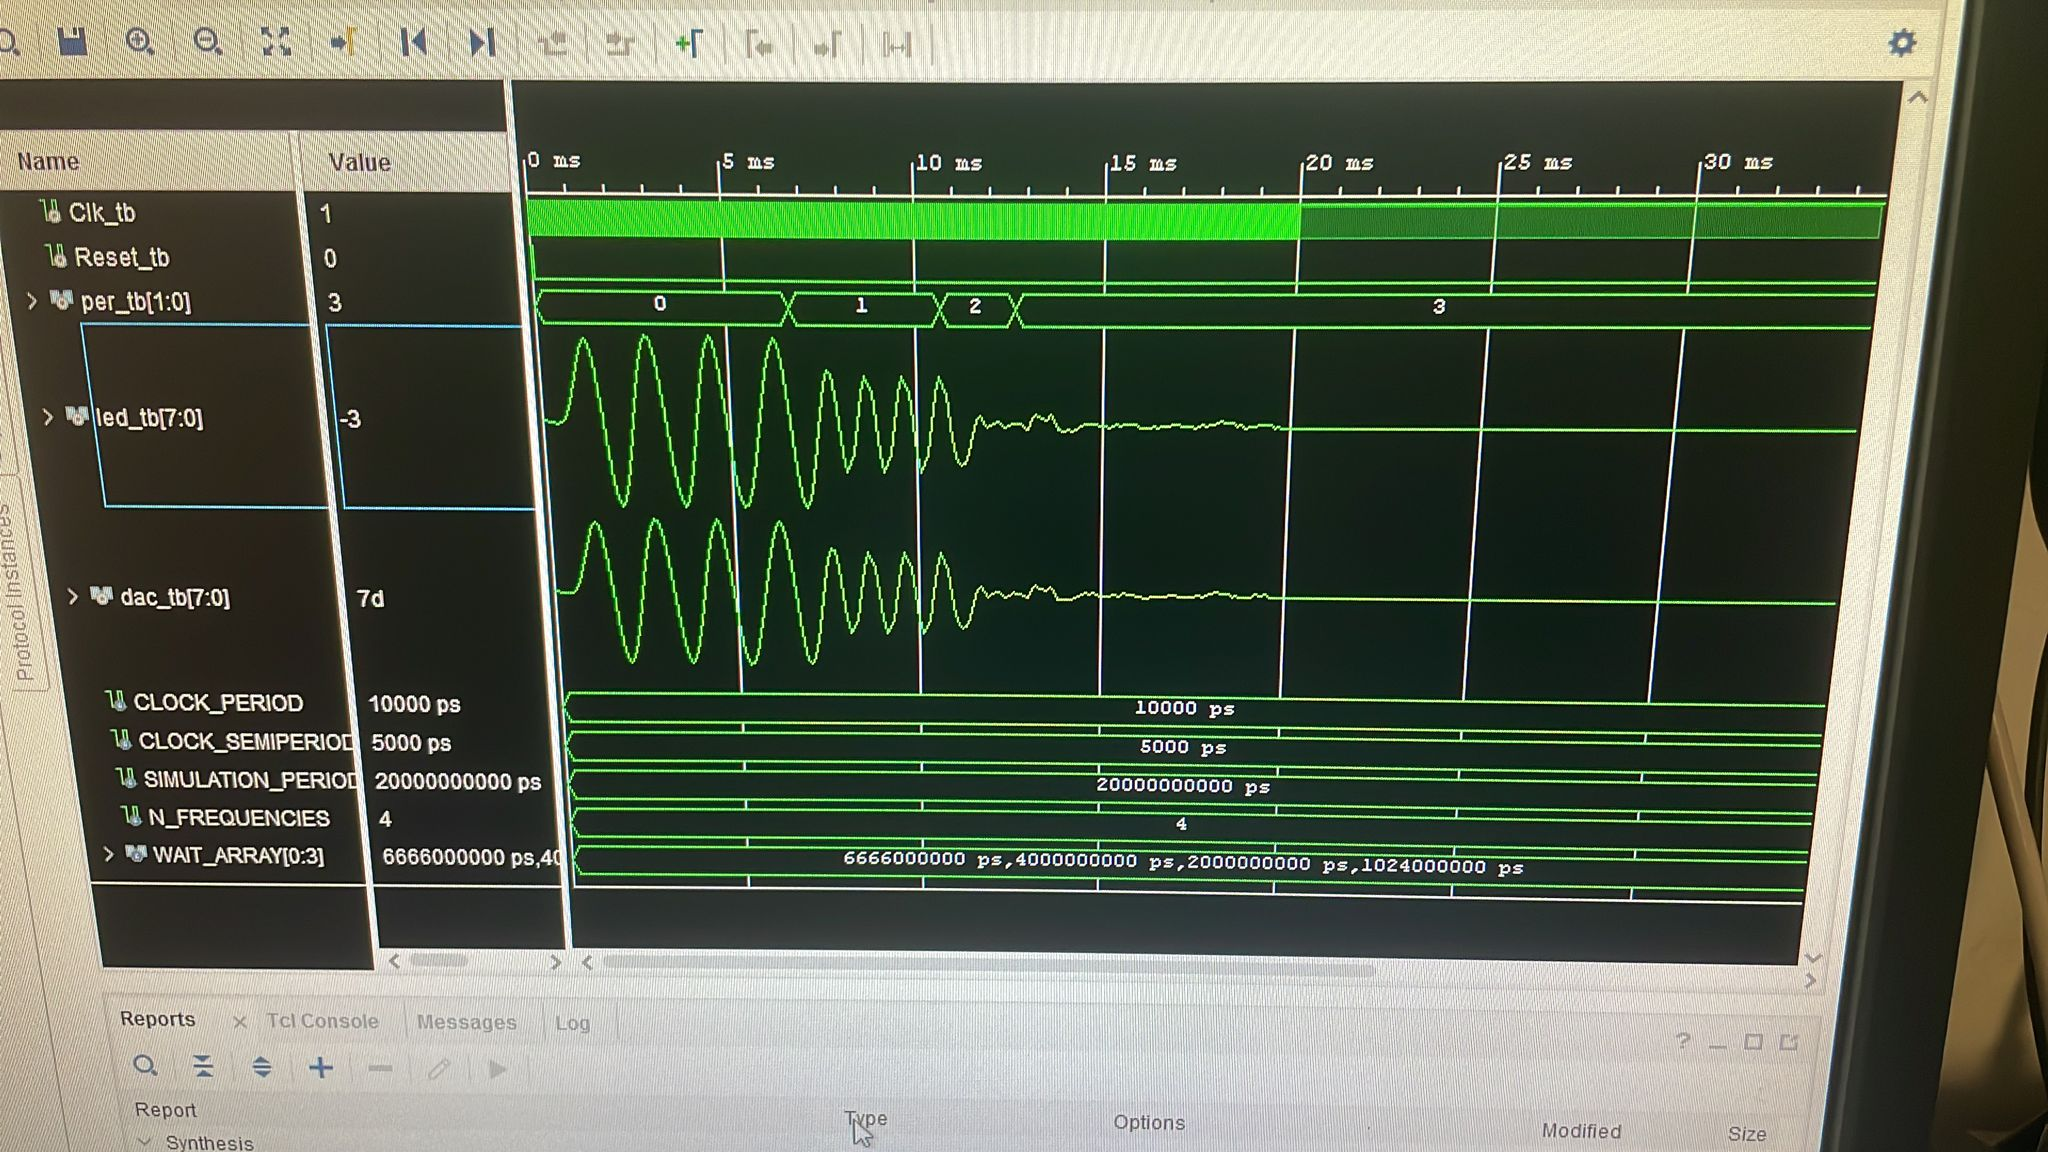
\includegraphics[width=.9\linewidth]{./img/simulation.jpg}
\end{center}
\section{Architectures}
\label{sec:org3f48db0}

\subsection{Parallel Architecture}
\label{sec:org995ef6a}



\subsection{One Flip-Flop Pipeline Architecture}
\label{sec:org8dc1fed}

\subsection{Two Flip-Flop Pipeline Architecture}
\label{sec:org831450f}
\section{Synthesis Results}
\label{sec:orgcf0f8ea}
\section{Conclusion}
\label{sec:org74c77a1}
\end{document}
